\section{Application to protoplanetary disks}\label{application} 
As an application of our results, we estimate where in a 
protoplanetary disk do the thermodynamic conditions allow the VSI to 
operate. Specifically, we consider the fundamental isothermal VSI, 
for which we can use the simple criterion Eq. \ref{iso_vsi_cond}. The
condition derived below may be considered as a sufficient condition for the VSI.  

In our disk models we have adopted a simple thermal relaxation
function in the energy equation. To connect our model with a realistic
disk, we consider the more physically-motivated form of the energy
equation with radiative cooling 
\begin{align}\label{real_energy}
\rho T \frac{DS}{Dt} = - \left(\nabla\cdot\bm{F} - Q_+\right), 
\end{align}
where the temperature $T$ is defined such that $P=\mathcal{R}\rho
T/\mu$, where $\mathcal{R}$ is the ideal gas constant and $\mu$ is
the mean molecular weight. In Eq. \ref{real_energy} $S$ is the
specific entropy,
\begin{align}
  S \equiv c_v\ln{\left(\frac{p}{\rho^{\gamma}}\right)} 
\end{align}
where $c_v \equiv \left(\gamma-1\right)^{-1}\mathcal{R}/\mu$ is the specific heat capcity at
constant volume, $D/Dt$ is the convective derivative, $\bm{F}$ is the
radiative flux, and $Q_+$ is a heating term such that an equilibrium
solution exists.  

Our aim is to relate the right hand side (RHS) of Eq. \ref{real_energy} to
the thermal relaxation time $t_c$ as used in our linear
calculations. To do so, we first consider separately perturbations
with radial lengthscales $L\equiv 2\pi/k_x\ll l_\mathrm{rad}$ and 
$L\gg l_\mathrm{rad}$, where      
\begin{align}\label{lrad}
  l_\mathrm{rad} \equiv \frac{1}{\kappa_d\rho} 
\end{align} 
is the photon mean-free-path and $\kappa_d$ is the (dust) opacity. 

\subsection{Newtonian cooling}
For $L\ll l_\mathrm{rad}$ the radiative cooling is given by {\bf (reference?)}
\begin{align}
\nabla\cdot\bm{F} = 4 \rho \kappa_d \sigma_s T^4,
\end{align}   
where $\sigma_s$ is the Stefan-Boltzmann constant. We choose the
heating term 
\begin{align}
  Q_+ = 4\rho\kappa_d\sigma_s T^{4}_{t=0}. 
\end{align}
Then Eq. \ref{real_energy} becomes
\begin{align}
  \frac{DP}{Dt} = -\gamma P \nabla\cdot\bm{v} -
  \frac{4P\kappa_d\sigma_s}{Tc_v}\left(T^4 - T_{t=0}^4\right). 
\end{align}
When linearized, the last term on the RHS becomes
\begin{align}
  -\frac{16\sigma_s}{c_v}\kappa_d T^3\left(\delta P -
    \frac{P}{\rho}\delta\rho\right). 
\end{align}
By comparing this expression with the linearized version of the energy
equation used in our calculations (Eq. \ref{energy_eq}), we identify 
\begin{align}\label{tc_newton_cool} 
  t_\mathrm{cool} = \frac{c_v}{16\sigma_s\kappa_dT^3}
\end{align}
as the thermal relaxation timescale for perturbation lengthscales
$L\ll l_\mathrm{rad}$. 

\subsection{Radiative diffusion}
For perturbation lengthscales $L\gg l_\mathrm{rad}$, let us assume that
temperature fluctuations are smoothed out by radiative diffusion. To
model this in linear theory, we choose the heating term such that
\begin{align}
  Q_+ - \nabla\cdot\bm{F} \equiv \nabla\cdot\left[k_\mathrm{rad}\nabla
    \left(T-T_{t=0}\right)\right], 
\end{align} 
where $k_\mathrm{rad}$ is the conduction coefficient to be defined
implicitly. Eq. \ref{real_energy} becomes
\begin{align}
  \frac{DP}{Dt} = -\gamma P \nabla\cdot\bm{v} + \frac{P}{\rho T
    c_v}\nabla\cdot\left[k_\mathrm{rad}\nabla\left(T-T_{t=0}\right)\right].     
\end{align}
When linearized, the last term on the RHS becomes
\begin{align}\label{diff_cool_proper}
  \frac{P}{\rho T c_v} \nabla\cdot\left(k_\mathrm{rad}\nabla\delta
    T\right). 
\end{align}
This, of course, fundamentally changes the linear problem by
introducing higher order derivatives. We defer a proper analysis of
this problem to a follow-up study. Here, we are interested in
order-of-magnitude estimates. We thus proceed by assuming vertical
derivatives can be neglected in Eq. \ref{diff_cool_proper} and write
\begin{align}\label{diff_cool_approx}
  \frac{P}{\rho T c_v} \nabla\cdot\left(k_\mathrm{rad}\nabla\delta
    T\right) &\to -\frac{k_\mathrm{rad}}{\rho
    c_v}k_x^2P\left(\frac{\delta T}{T}\right)\notag\\
  &\equiv -\eta k_x^2 \left(\delta P - \frac{P}{\rho}\delta\rho\right), 
\end{align}
%we are interested in radially-thin perturbations  
where $\eta=k_\mathrm{rad}/\rho c_v$ is the diffusion coefficient and
is given in terms of physical disk parameters as 
\begin{align}\label{eta_def}
  \eta = \frac{16\sigma_s T^3}{3\kappa_d\rho^2 c_v}. 
\end{align}
From Eq. \ref{diff_cool_approx} we identify the thermal relaxation
time for diffusion as 
\begin{align}\label{tc_diff_cool} 
  t_\mathrm{diff} = \frac{1}{\eta k_x^2}\equiv \frac{\Omega_k^{-1}}{\hat{\eta}\khat^2}, 
\end{align}
where $\hat{\eta} = \eta/H_\mathrm{iso}^2\Omega_k$ is the 
dimensionless diffusion coefficient defined for convenience, and is
approximately 
\begin{align}\label{diff_coeff_dimensionless}
  \hat{\eta} \simeq  \frac{16\sigma_s T^3}{3\kappa_d\Sigma^2
    c_v\Omega_k}. 
\end{align}

\subsection{Toy model for realistic thermal relaxation}
To unify $t_\mathrm{cool}$ and $t_\mathrm{diff}$, we define the
effective thermal relaxation timescale in linear theory as
\begin{align}\label{tc_def}
  t_c &\equiv t_\mathrm{cool} + t _\mathrm{diff} =
  \frac{l_\mathrm{rad}^2}{3\eta} + \frac{1}{\eta k_x^2},  
\end{align}
where the relation between $t_\mathrm{cool}$, $l_\mathrm{rad}$ and
$\eta$ can be inferred from Eq. \ref{lrad}, Eq. \ref{tc_newton_cool}
and Eq. \ref{eta_def}. Eq. \ref{tc_def} is a simple prescription so
that for small scales (large $k_x$), $t_c\to t_\mathrm{cool}$, while
for large scales (small $k_x$), $t_c\to t_\mathrm{diff}$. 

The dimensionless thermal relaxation time $\beta$ is then
\begin{align}\label{real_beta}
  \beta \equiv t_c\Omega_k =
  \frac{1}{\hat{\eta}}\left(\frac{l_\mathrm{rad}^2}{3H_\mathrm{iso}^2}
    + \frac{1}{\khat^2}\right)  \simeq
  \frac{1}{\hat{\eta}}\left(\frac{1}{3\kappa_d^2\Sigma^2} 
    + \frac{1}{\khat^2}\right).
\end{align}

\subsection{Evaluation for a fiducial disk model}
We evaluate Eq. \ref{real_beta} for the protoplanetary disk model
described in \cite{chiang10} and summarized in Appendix \ref{mmsn}
(where an opacity model is also chosen). Defining $\zeta\equiv
r/\mathrm{AU}$, we find Eq. \ref{real_beta} becomes
\begin{align}\label{beta_mmsn}
\beta =
\frac{4.4\times10^5}{\mu(\gamma-1)}\left(\frac{\hat{\kappa}_d\hat{\Sigma}^2}{\hat{T}}\right)\zeta^{-57/14}\left(\frac{8.3\times10^{-9}}{\hat{\kappa}_d^2\hat{T}^4\hat{\Sigma}^2}\zeta^{33/7}+\frac{1}{\khat^2}\right).  
\end{align}
We also evaluate the criterion Eq. \ref{iso_vsi_cond} for the fiducial
disk model, 
\begin{align}\label{bcrit_mmsn}
  \beta_\mathrm{crit} = \frac{9.4\times10^{-3}}{(\gamma
    -1)}\zeta^{2/7},
\end{align}
and we recall $\beta < \beta_\mathrm{crit}$ permits the fundamental 
isothermal VSI to operate. 

In Fig. \ref{mmsn_bcrit_bcool} we plot Eq. \ref{beta_mmsn} and
Eq. \ref{bcrit_mmsn} for the MMSN with $\mu = 2$ and
$\gamma=1.4$. Although it is possible to satisfy
$\beta<\beta_\mathrm{crit}$ at small radii by choosing a sufficiently
large $\khat$, our linear calculations suggest growth rates eventually
decay as $\khat\to\infty$. We thus restrict our attention to
$\khat\lesssim 10^2$. 

Fig. \ref{mmsn_bcrit_bcool} suggests that the fundamental isothermal
VSI can operate in the outer parts of the MMSN at radii on the order
of tens of AU. However, the thermal relaxation time $\beta$ is not
much shorter than $\beta_\mathrm{crit}$, so the VSI may be
weak.   

\begin{figure}
  \includegraphics[width=\linewidth]{figures/bcrit_mmsn}  
  \caption{Dimensionless thermal relaxation timescales $\beta$ in the MMSN
    using Eq. \ref{beta_mmsn} for three values of the 
    perturbation radial wavenumber: $\khat=1$ (dotted), $\khat=10$
    (dashed) and $\khat=100$ (dashed-dot). The relaxation timescale
    $\beta_\mathrm{crit}$, below which the fundamental isothermal VSI
    operates, is shown as the solid line. 
    \label{mmsn_bcrit_bcool}}   
\end{figure}  

\subsection{Numerical example}
Consider  the MMSN at $r=30\mathrm{AU}$, with $\gamma=1.4$ and
$\mu=2$. Eq. \ref{mmsn_epsilon} gives $\epsilon \simeq
0.058$ which implies, using Eq. \ref{bcrit_mmsn}, a critical 
relaxation timescale of  
\begin{align*}
  \beta_\mathrm{crit} \simeq 0.062. 
\end{align*} 
To estimate a thermal relaxation timescale, we set $\khat=20$ 
in Eq. \ref{beta_mmsn} to obtain 
\begin{align*}
  \beta \simeq 0.042.
\end{align*}
(In fact, Fig. \ref{mmsn_bcrit_bcool} shows that $\beta$  is not
sensitive to $\khat$ at $r=30\mathrm{AU}$, provided that $\khat\gg1$.)
The disk supports the fundamental isothermal VSI, but only
marginally. Using the above value of $\beta$, MMSN disk parameters and
$\khat=20$ in our linear code, we find a  
growth rate of 
\begin{align*}
  \nu = 3.3\times10^{-3}\Omega_k.
\end{align*}
This corresponds to a characteristic growth time of $t_g\sim 50$
orbits. This mode was found to be the most unstable for
$\khat=20$. 
% and
% physically acceptable -> other modes
% are crazy  

We also solved the linear problem with varying $\khat$  
and $\beta$ determined by Eq. \ref{beta_mmsn}. We find the most
unstable wavenumber occurs at $\khat\simeq60$ with $\nu\simeq
3.6\times10^{-3}\Omega_k$, i.e. only slightly faster than $\khat=20$.   
However, the eigenfunctions for large $\khat$ were found to have large
amplitude oscillations near the vertical boundaries. This is shown in
Fig. \ref{mmsn_eigenW}. These modes may not be important since they
mostly affect the disk atmosphere where there is little mass. 

\begin{figure}
  \includegraphics[width=\linewidth,clip=true,trim=0cm 1.75cm 0cm 0cm]{figures/eigenvectorW_mmsnkx20.ps}
  \includegraphics[width=\linewidth,clip=true,trim=0cm 0cm 0cm 0cm]{figures/eigenvectorW_mmsnkx60.ps}
  \caption{Most unstable VSI modes in the MMSN at
    $r=30\mathrm{AU}$. The eigenfunction $W$ for $\khat=20$ (top) and
    $\khat=60$ (bottom) are shown. The real (imaginary) part of $W$
    is plotted as the solid (dotted) lines.\label{mmsn_eigenW}}  
\end{figure}

% only find one unstable mode -> close to marginal 
% larger kx 